% kuleuventheme2 by Janez Kren, September 2017, janez.kren@kuleuven.be, based on:
% kuleuventheme 1.3 by Roland Pastorino, 2013 roland.pastorino@kuleuven.be / www.rolandpastorino.com

\documentclass[11pt,t]{beamer}
\usetheme{kuleuven2}	%THEME OPTIONS for LOGO: kul (default), kulak, lrd,    ; OPTIONS for TITLE PAGE: normal (default), sedes


%%% OTHER SETTINGS
\usefonttheme[onlymath]{serif}			% math font with serifs, delete to make it sans-serif
\setbeamertemplate{footline}[body] 		% delete this line to remove footline bar on all frames
%\usepackage[orientation=landscape,size=custom,width=16,height=9,scale=0.5,debug]{beamerposter} %enable for widescreen 16:9 ratio
%\titlegraphic{ \includegraphics[width=.2\paperwidth]{mytitlepagepic.png} } %optional title page image


%%% ADDED PACKAGES:
\usepackage[dutch]{babel}
\usepackage{amsfonts}
\usepackage{amssymb}


%%% TITLE PAGE INFO:
\title[Tussentijdse presentatie]{Visie voor semantische robotnavigatie in ziekenhuisgangen} %[]] will appear in footline
\subtitle{Tussentijdse presentatie}

\author{Olivier Van den Eede}
\institute{KU Leuven - De Nayer}
\date{Januari 2019}


\begin{document}
\csname beamer@calculateheadfoot\endcsname %recalculate head and foot dimension

 %%
 %%  0. TITLE PAGE and TABLE OF CONTENT
 %%
% Title page
\begin{frame}[plain,noframenumbering]
	\titlepage
\end{frame}
	

% Table of Contents
\begin{frame}{Inhoud}
	\hfill	{\large \parbox{.961\textwidth}{\tableofcontents[hideothersubsections]}}
\end{frame}



 %%
 %%  SECTION 1 - Probleemstelling
 %%
\section{Probleemstelling}
\begin{frame}[fragile]{Probleemstelling}
	\begin{itemize}
		\item Personeelstekorten
		\item Hoge werkdruk voor zorgpersoneel
		\item Textiellogistiek en goederenstroom
		\item Automatisatie moeilijk door infrastructuur en bestaand logistiek materiaal
	\end{itemize}
\end{frame}

\begin{frame}[fragile]{Mogelijke oplossing}
	\begin{itemize}
		\item Autonoom Geleid Voertuig (AGV)
		\item Zelfstandige navigatie doorheen ziekenhuisgangen
		\item Voertuig uitgerust met sensoren en een RGB camera
		\item Semantische kaart voor navigatie
	\end{itemize}
\end{frame}

\begin{frame}[fragile]{Doel masterproef}
	\begin{itemize}
		\item Onderzoeken aanwezige objecten/features in ziekenhuisgangen
		\item Zoeken van gepaste beeldverwerkingstechnieken
		\item Objectdetectie gebruiken voor lokalisatie op de kaart
		\item Op basis van kaart en gekende startlocatie navigeren naar eindpunt
	\end{itemize}
\end{frame}



 %%
 %%  SECTION 2 - Literatuurstudie
 %%
 \section{Literatuurstudie}
 \begin{frame}[fragile]{Indoor navigatie & visie}
	\begin{itemize}
		\item Oudere technieken op basis van RGB camera's
		\item Moderne technieken werken met RGB-D camera's
		\item Beperken tot RGB camera
	\end{itemize}
 \end{frame}

 \begin{frame}[fragile]{Object detectie}
	\begin{itemize}
		\item Traditionele technieken
		\begin{itemize}
			\item Template matching
			\item Local feature matching
		\end{itemize}
		\item Convolutional neural network (CNN)
	\end{itemize}
 \end{frame}

%  \begin{frame}[fragile]{Object tracking}
% 	\begin{itemize}
% 		\item 
% 	\end{itemize}
%  \end{frame}

 \begin{frame}[fragile]{Image segmentatie}
	\begin{itemize}
		\item Onderscheid tussen vloeren en wanden
		\item K-means op textuur en kleur
		\item Reflecties en overbelichting belangrijke factor
		\item Segmentatie op basis van kleur tussen gedetecteerde lijnen
		\item Segmentatie CNN
	\end{itemize}
 \end{frame}



 %%
 %%  SECTION 3 - Reeds gerealiseerda
 %%
\section{Reeds gerealiseerd}
\begin{frame}[fragile]{Pictogram detectie}
	Doel
	\begin{itemize}
		\item Segmentatie op basis van hue
		\item Local feature matching met SIFT
	\end{itemize}

	Problemen
	\begin{itemize}
		\item Grote verschillen in belichting
		\item Slecht beeldmateriaal
	\end{itemize}

	\begin{figure}
		\centering
		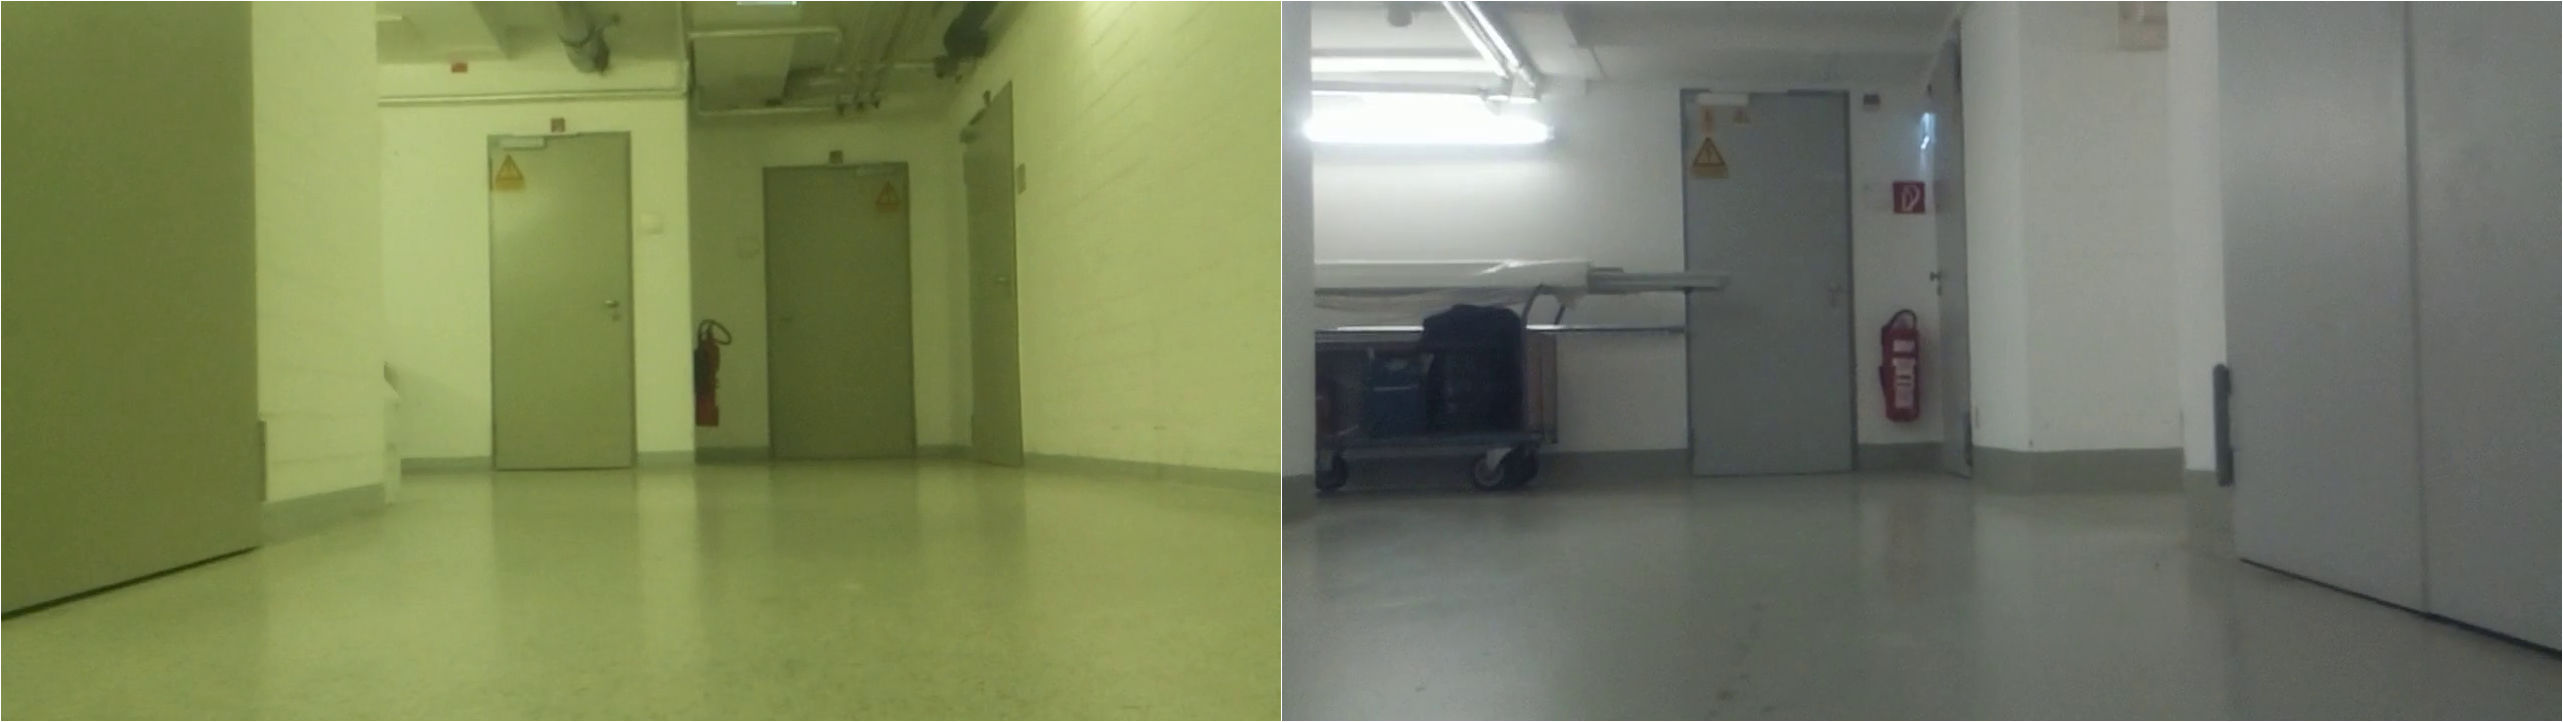
\includegraphics[width=0.6\textwidth]{graphics/kleurverschil.png}
		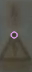
\includegraphics{graphics/sift_detectie.png}
		\flushleft
	\end{figure}
\end{frame}

\begin{frame}[fragile]{Object detectie met CNN}
	\begin{itemize}
		\item Annotatie beeldmateriaal met CVAT
		\item Conversie CVAT output naar YOLO input
		\item Trainen CNN voor detectie van 4 objecten
	\end{itemize}
\end{frame}

\begin{frame}[fragile]{Object detectie met CNN}
	\begin{figure}
		\centering
		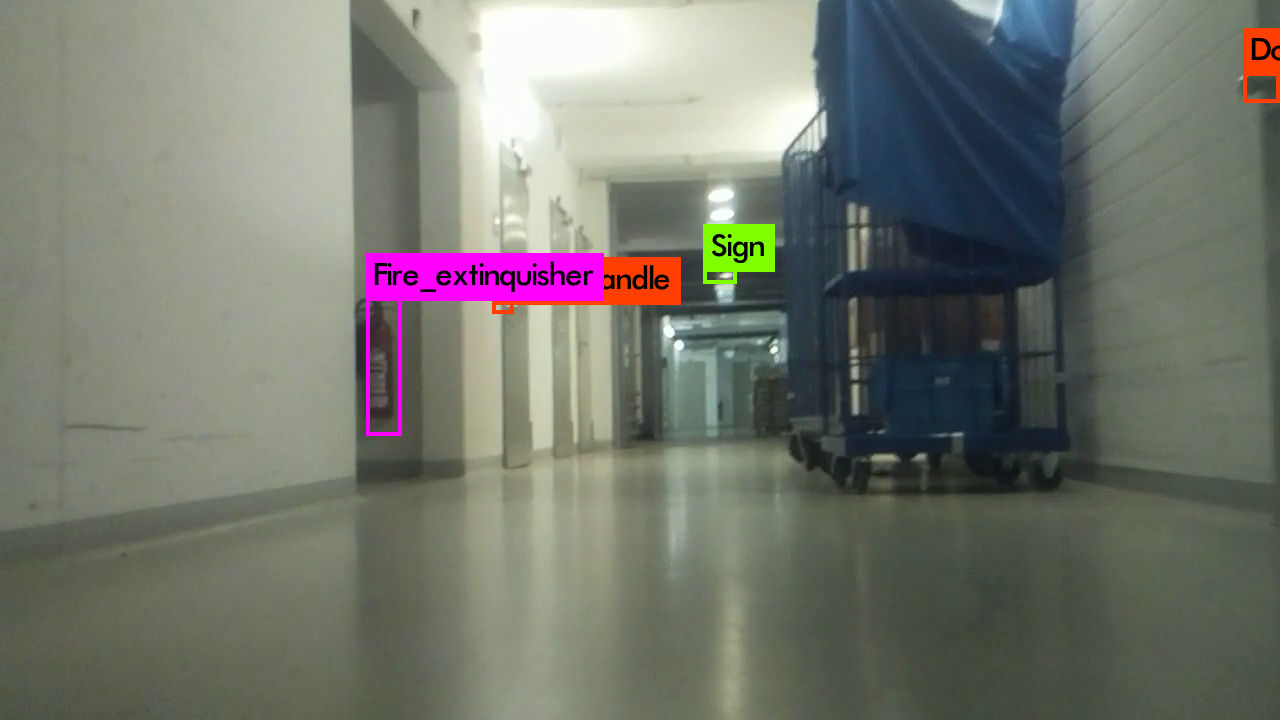
\includegraphics[width=0.6\textwidth]{graphics/yolo_detectie1.jpg}
		\flushleft
	\end{figure}
\end{frame}

\begin{frame}[fragile]{Object detectie met CNN}
	\begin{figure}
		\centering
		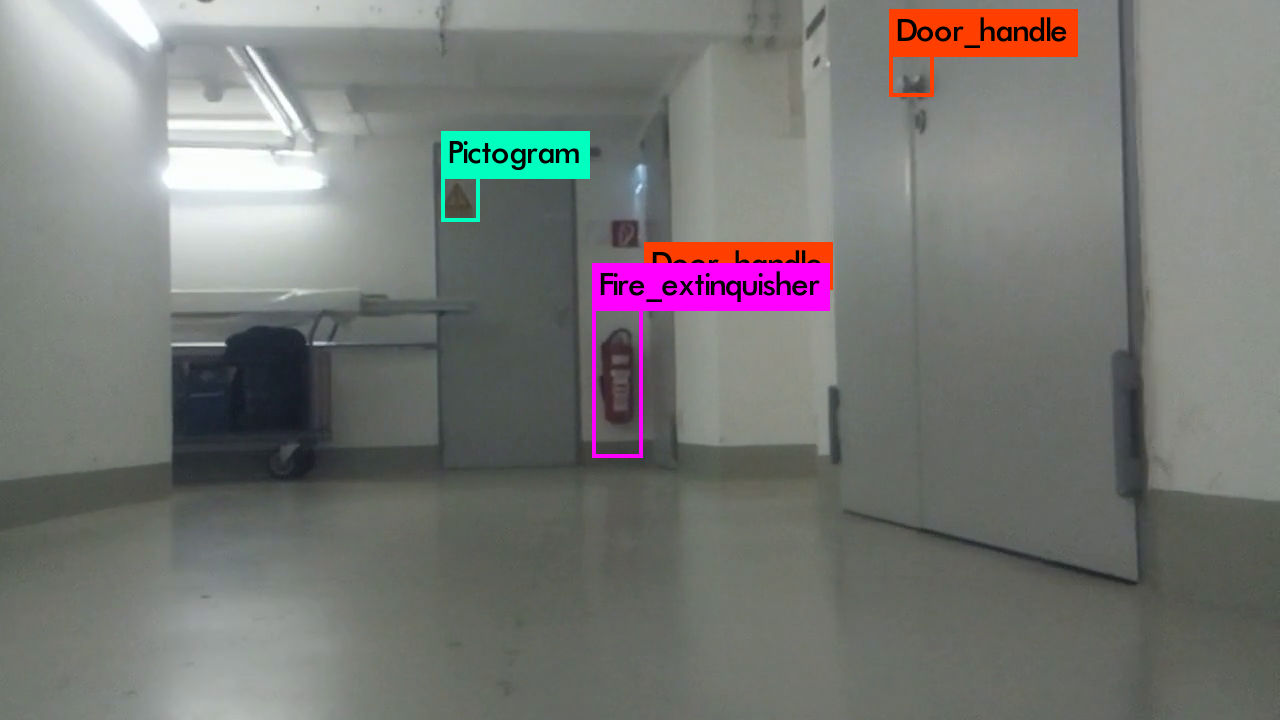
\includegraphics[width=0.6\textwidth]{graphics/yolo_detectie2.jpg}
		\flushleft
	\end{figure}
\end{frame}

\begin{frame}[fragile]{Image segmentation}
	\begin{itemize}
		\item SegNet segmentatie netwerk
		\item ResNet gebaseerd segmentatie netwerk (getraind op dataset met indoor scenes en gangen)
		\item Getest zonder hertraining
	\end{itemize}

	\begin{figure}
		\centering
		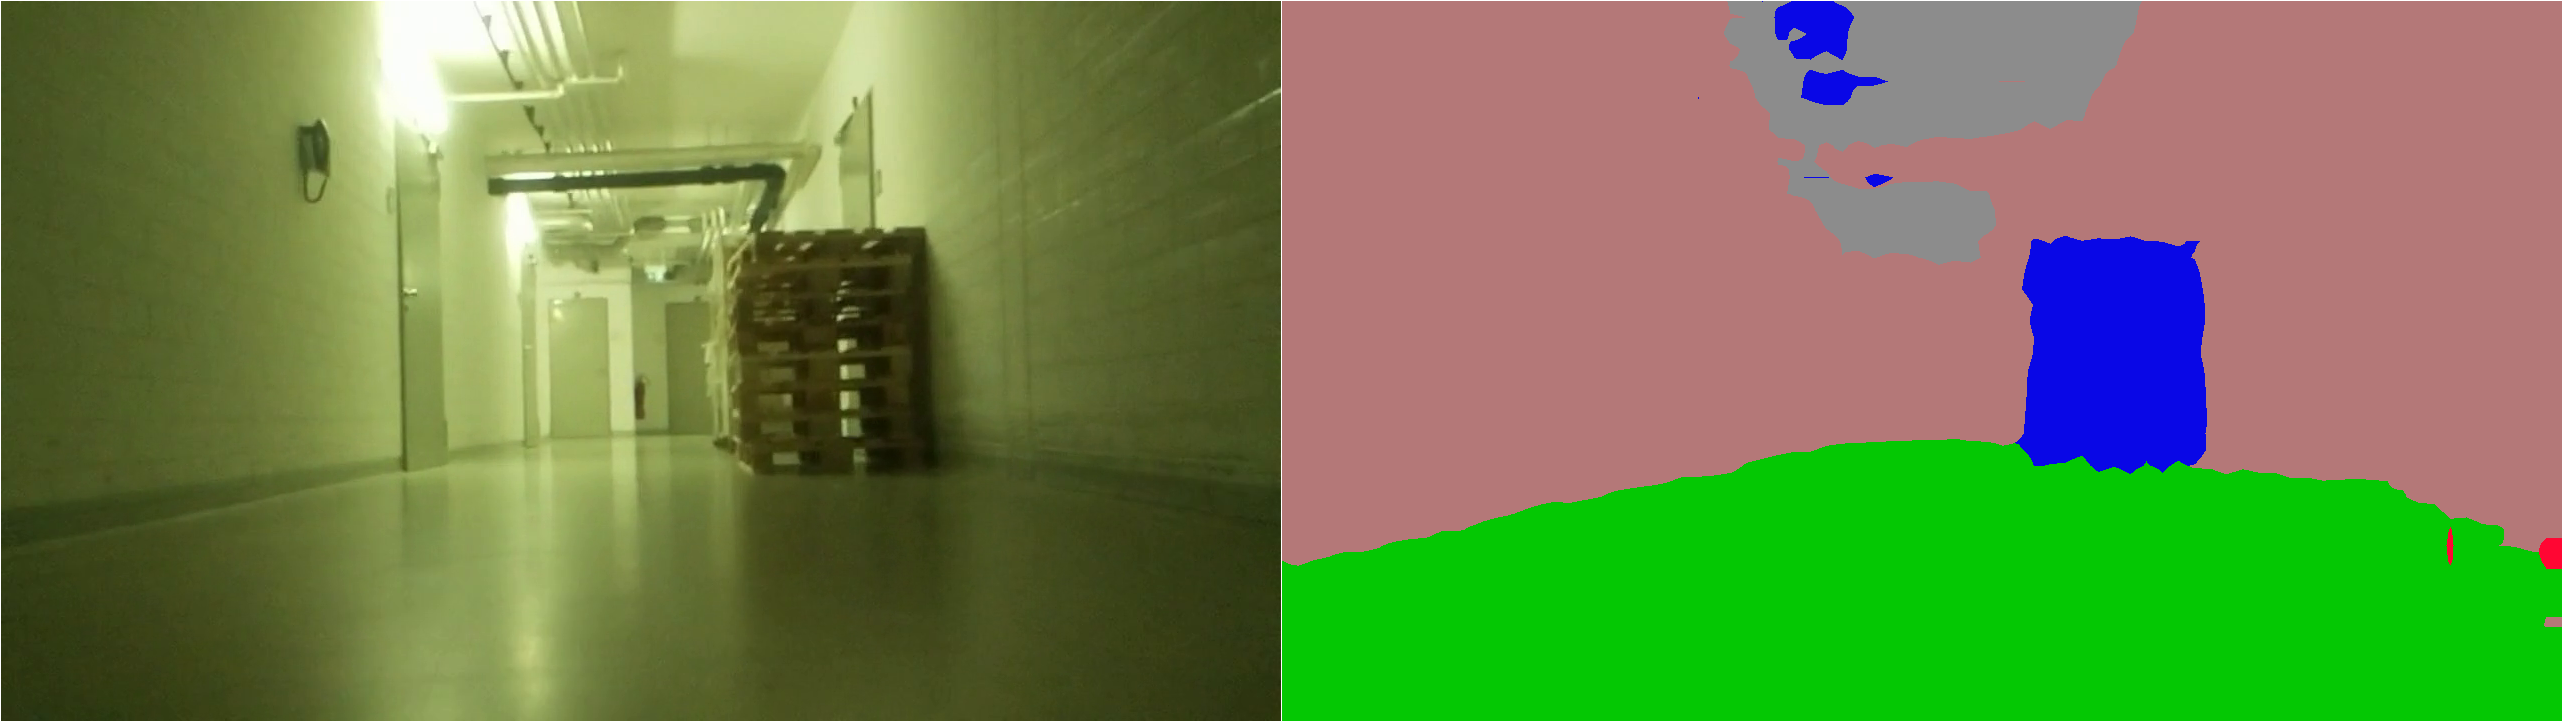
\includegraphics[width=0.6\textwidth]{graphics/resnet_segmentatie.png}
		\flushleft
	\end{figure}
\end{frame}

 %%
 %%  SECTION 4 - Planning
 %%
 \section{Verder verloop}
 \begin{frame}[fragile]{Verder verloop}
	\begin{itemize}
		\item Werken met nieuw beeldmateriaal
		\item Verder uitwerken object detectie met YOLO
		\item Verder onderzoek naar segmentatie netwerken
		\item Objectdetectie/tracking koppelen aan kaart
		\item Lokalisatie op basis van de kaart
	\end{itemize}
 \end{frame}

\begin{frame}[c,plain,noframenumbering]
\begin{tikzpicture}[remember picture,overlay]
\fill[fill=kul-blue]
    (current page.south east)  rectangle  ([shift={(0,-0.1\paperheight)}]current page.north west)   ;
\end{tikzpicture}

\centering
\textcolor{white}{Vragen?}
\end{frame}


\end{document}